\documentclass{webofc}
\usepackage[varg]{txfonts}
% review
%\usepackage[textwidth=120]{todonotes}
%\usepackage{color}
\usepackage{subcaption}

\begin{document}

\title{Application of Turchin's method of statistical regularization}
\author{\firstname{Mikhail} \lastname{Zelenyi}\inst{1,2}\fnsep\thanks{\email{mihail.zelenyy@phystech.edu}} \and
    \firstname{Mariia} \lastname{Poliakova}\inst{1,2} \and \firstname{Alexander} \lastname{Nozik}\inst{1,2}\fnsep\thanks{\email{altavir@gmail.com}} \and \firstname{Alexey} \lastname{Khudyakov}\inst{1}\fnsep\thanks{\email{alexey.skladnoy@gmail.com}}  
    }
%
\institute{Institute for Nuclear Research RAS
    \and
    Moscow Institute of Physics and Technology
}
\abstract{%
    During analysis of experimental data, one usually needs to restore a signal after it has been convoluted with some kind of apparatus function. According to Hadamard's definition this problem is ill-posed and requires regularization to provide sensible results. In this article we describe an implementation of the Turchin's method of statistical regularization based on the Bayesian approach to the regularization strategy.
}
%
\maketitle

\section{Introduction}

\subsection{Problem}

Consider the usual situation: detector measures a signal ($\varphi(x)$) and produces observed data ($f(y)$) via convolution with its own apparatus function ($K(x,y)$). The resulting observed data $f(y)$ contains a random noise factor both from initial statistical uncertainty of $\varphi(x)$ and additional noise from measurement procedure. In order to reconstruct initial signal, one needs to solve Fredholm equation of 1-st kind:
\begin{equation}
\label{eq-01}
    f(y) = \int dx~ K(x,y)\varphi(x),
\end{equation}
but this equation is ill-possed: a small error in the measurement of $f(y)$ leads to big instability of $\varphi(x)$. 

\subsection{Solution}

Solving such ill-possed problems requires additional operation called regularization. It means we need to introduce additional information to problem well-posed one. The idea of statistical regularization~\cite{Turchin, Turovceva} is to look on the problem from the point of view of Bayessian statistics approach: unknown statistical value $\varphi(x)$ could be reconstructed using  measured value $f(y)$, the model ($K(x,y)$) and some prior information about $\varphi(x)$ behavior. Main features of statistical regularization:
\begin{itemize}
    \item Based on Bayesian approach and decision theory (choice theory).
    \item It's able to accommodate various forms of prior information, such as
      smoothness, constraints on boundary conditions, non-negativity, etc.
    \item It allows estimation of errors for reconstructed function $\varphi$
    \item Gives clear data-driven procedure for choice of regularization
      strength.
\end{itemize}

While the idea of the regularization was proposed a long time ago, it was not published in the journal with sufficient visibility and therefore left unknown to the broad scientific auditory. The aim of this work is both to reconstruct the initial work (create a modern implementation for described algorithms), and study its performance under different conditions.

Since original work is very hard to find and was published only in Russian language, we will present the short description of the method.

\section{Description of statistical regularization's method}

\subsection{Strategy}\label{sec:theory:strat}
Consider eq.~\ref{eq-01} in operator form:
\begin{equation}
	\label{eq-02}
    \hat{K}\varphi = f.
\end{equation}
According to statistical decision theory (\cite{james2006statistical}), one can define a reconstruction strategy  $\hat{\varphi} = \hat{S}[f]$, which uses a prior information. Good strategy minimize an impact of prior information (which could be wrong). That could be achieved by introducing the loss-function:
\begin{equation*}
	L(\varphi,\hat{S}[f]) = ||\varphi-\hat{S}[f])||_{L_2},
\end{equation*}
For this loss-function:
\begin{equation}
	\label{eq:opt}
	\hat{S}[f] = E[\varphi|f] = \int \varphi P(\varphi|f)d\varphi
\end{equation}
Strategy depend on a prior information $P(\varphi)$:
\begin{equation*}
	P(\varphi|f)= \frac{P(\varphi)P(f|\varphi)}{\int d\varphi P(\varphi)P(f|\varphi)} 
\end{equation*}
Errors of solution:
\begin{equation*}
	D(x_1,x_2)  = E[\varphi(x_1) - \hat{S}[f](x_1)][\varphi(x_2) - \hat{S}[f](x_2)]
\end{equation*}
Let us consider what a prior information can we use? 

\subsection{A prior information}\label{sec:theory:aprior}

We expect that $\varphi$ is relatively smooth and doesn't contain wild
oscillations which, for example, we usually produce in use naive least squares. Common way of measuring
function's smoothness is $\langle\varphi,\hat{\Omega}\varphi\rangle$, where
$\hat{\Omega}=|\frac{d^2}{dx^2}\left\rangle\right\langle\frac{d^2}{dx^2}|$.
At the same time we want to minimize information content of prior. 

Reasonable choice is ensemble of functions with average smoothness $\omega$ which
maximizes Shannon entropy (or is equivalent to minimize that value of Shannon's information, which we add to solution). Which means we need to maximize:

\begin{equation*}
  H[P(\varphi)] = -\int \ln{P(\varphi)} P(\varphi) d\varphi
\end{equation*}

Subject to constraints:

\begin{equation}
  \int P(\varphi) d\varphi = 1
  \qquad\mbox{and}\qquad
  \int \langle \varphi,\hat{\Omega}\varphi \rangle P(\varphi) d\varphi = \omega,  
  \label{eq-smoothness}
\end{equation}

The resulting prior probability density for the Gaussian random process:
\begin{equation}
  P(\vec{\varphi}|\alpha) = \frac{\det(\alpha\Omega)^{1/2}}{(2\pi)^{N/2}} 
  \exp\left(-\frac{1}{2}\langle\vec{\varphi},\alpha\Omega\vec{\varphi}\rangle\right),
  \label{eq-prior}
\end{equation}
where $\alpha = \alpha(\omega)$~--- parameter of smoothness. In result, we get $\alpha$-depend solution $\hat{S}_{\alpha}[f]$ and now we have problem of picking $\alpha$. In rare cases we can select $\alpha$ manually using known empirical smoothness, but we proposal another way. Information about its value almost never available so we could consider it random variable as well. This yields us hierarchical Bayes model $P(f,\varphi,\alpha) = P(f|\varphi)P(\varphi,\alpha)P(\alpha)$.
Since we don't have any information about $\alpha$ we chose hyperprior $P(\alpha)$ to be flat. Now we have several options to pursue. In general case, we can use fully Bayesian approach  and compute solution to marginalize by $\alpha$ and to use eq. ~\ref{eq:opt}:
    \begin{equation}\label{eq:varAposteriorAlpha}
    P(\varphi) = \int P(\varphi|\alpha) P(\alpha)~d\alpha 
    \end{equation}
or,  to marginalize by $\varphi$ and to integrate by $P(\alpha|f)$:
    \begin{equation}
    P(\alpha|f) \sim \int d\varphi~P(f|\varphi)P(\varphi|\alpha)P(\alpha)
    \qquad\mbox{and}\qquad
    \hat{S}[f] =\frac{1}{Norm} \int d\alpha \hat{S}_{\alpha}[f] P(\alpha|f)
    \label{eq:solveAposteriorAlpha}
    \end{equation}
    using MCMC for sampling $\varphi$ and $\alpha$ (for Gaussian errors it could be reduced to numerical integral). In particular case we can simplify calculations by using following approximations. Also if distribution $P(\alpha|f)$ is narrow, we can pick $\alpha$ corresponding to most probable $\alpha_0$ and use $P(\varphi|\alpha_0)$ as prior. This is called empirical Bayes. For our problem it produces almost identical results.
    
Derivation above assumed that $\Omega$ if positive definite. It possible to
accommodate singular $\Omega$. Then $\det$ in~(\ref{eq-prior}) should be
replaced with pseudodeterminant. Positive definiteness is desirable since
regularization is guaranteed to work only for non-singular $\Omega$ and singular
or even near-singular $\Omega$ may and likely will cause numerical problems.

Also note that $\Omega$ we use is singular since $\varphi = kx + b$ will have
smoothness equal to zero. One way fix it is to fix value of $\varphi$ to 0 and
boundaries or to put priors on values on
boundaries\cite{calvetti2006aristotelian}. In that case $\alpha\Omega$
in~(\ref{eq-prior}) should be replaced with $\sum_i\alpha_i\Omega_i$ where
different $\Omega_i$ corresponds to smoothness, boundary values etc.

Also it's possible to add any other prior information about function. For
example it possible to add non-negativity:

\begin{equation*}
    P(\varphi) \sim P_{\alpha}(\varphi)P(\varphi(x) > 0)
\end{equation*}


\subsection{Discretization}

In order to find numerical solution, one need to go from continuous functions in eq.~\ref{eq-02} to discrete matrix form:
\begin{equation}\label{eq:algebr}
	\begin{gathered}
      \varphi(x) = \sum \limits_n \varphi_n T_n(x),
      \qquad\mbox{and}\qquad
      K_{mn} = (\hat{K}T_n(x))(y_m),\\
      \Omega_{ij} = \int\limits_a^b \left(\frac{d^pT_i(x)}{dx}\right)\left(\frac{d^pT_j(x)}{dx}\right)dx,\\
      D[\varphi(x)] = D[\sum \limits_n \varphi_n T_n(x)] = \sum\limits_{i,j} \varphi_i\varphi_j cov(T_i(x), T_j(x)),\\
      \vec{f} = K\vec{\varphi},
    \end{gathered}
\end{equation}
where $T_n(x)$ - some basis in function space. For example, cubic spline, Fourier series and Legendre polynomials.

\subsection{Solution for Gaussian distributed noise}

The most common experimental case of noise distribution is normal (or Gaussian) distribution:
\begin{equation}	\label{eq:gaussP}
	P\left(\vec{f}|\vec{\varphi}\right) = \frac{1}{(2\pi)^{M/2}|\Sigma|^{1/2}} 
    \exp\left(-\frac{1}{2}(\vec{f} - K\vec{\varphi})^T\Sigma^{-1}(\vec{f} - K\vec{\varphi})\right)
\end{equation}
Using  the most probable $\alpha$, one can get the best solution in a simple form.
\begin{equation} \label{eq:analit_solv}
	\hat{S}_{\alpha}[\vec{f}] = (K^T\Sigma^{-1}K+\alpha\Omega)^{-1}K^T\Sigma^{-1T}\vec{f},
\end{equation}
\begin{equation} \label{eq:analit_var}
	\texttt{cov}_{\alpha}(\varphi_m, \varphi_n) = ||(K^T\Sigma^{-1}K+\alpha^*\Omega)^{-1}||_{mn}
\end{equation}
For definition $\alpha$, we use a posterior probability, which is calculated using Bayes' rule: 
\begin{equation}
	\label{eq:alphaaposter}
	P(\alpha|\vec{f}) = C \alpha^{\frac{Rg(\Omega)}{2}}\sqrt{|(B+\alpha\Omega)^{-1}|}\exp(-\frac{1}{2}b^{T}B^{-1}b)\exp(\frac{1}{2}b^{T}(B+\alpha\Omega)^{-1}b),
\end{equation}
where norming factor $C$  doesn't depend on $\alpha$. If we want to get more accurate solution, we should average solution over this posterior probability as it is describe in integrals ~\ref{eq:solveAposteriorAlpha}.

\section{Application}

\begin{figure}[ht!]
	\begin{subfigure}[b]{0.5\textwidth}
    	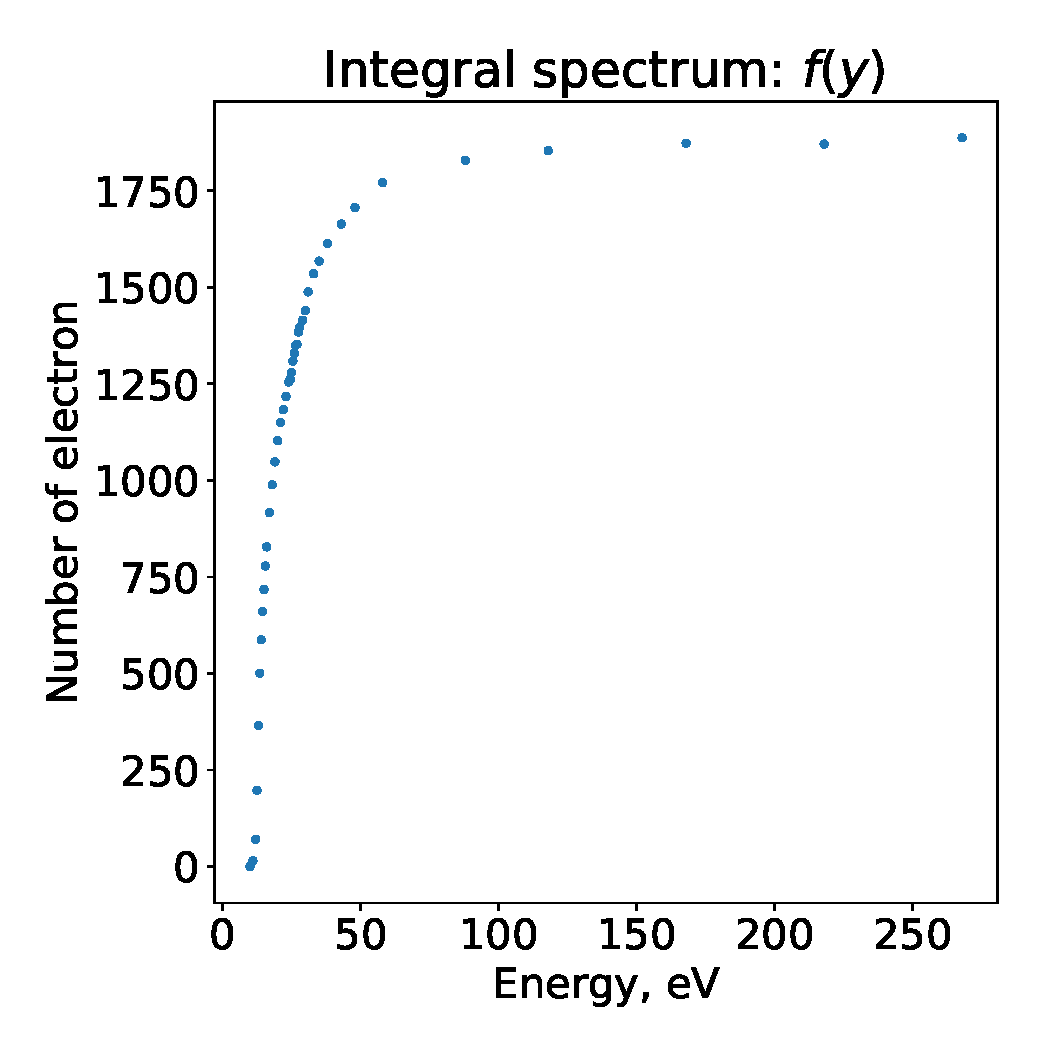
\includegraphics[width=0.95\linewidth]{image/fig01}
        \caption{}
        \label{pic-01-a}
    \end{subfigure}
	~
    \begin{subfigure}[b]{0.5\textwidth}
		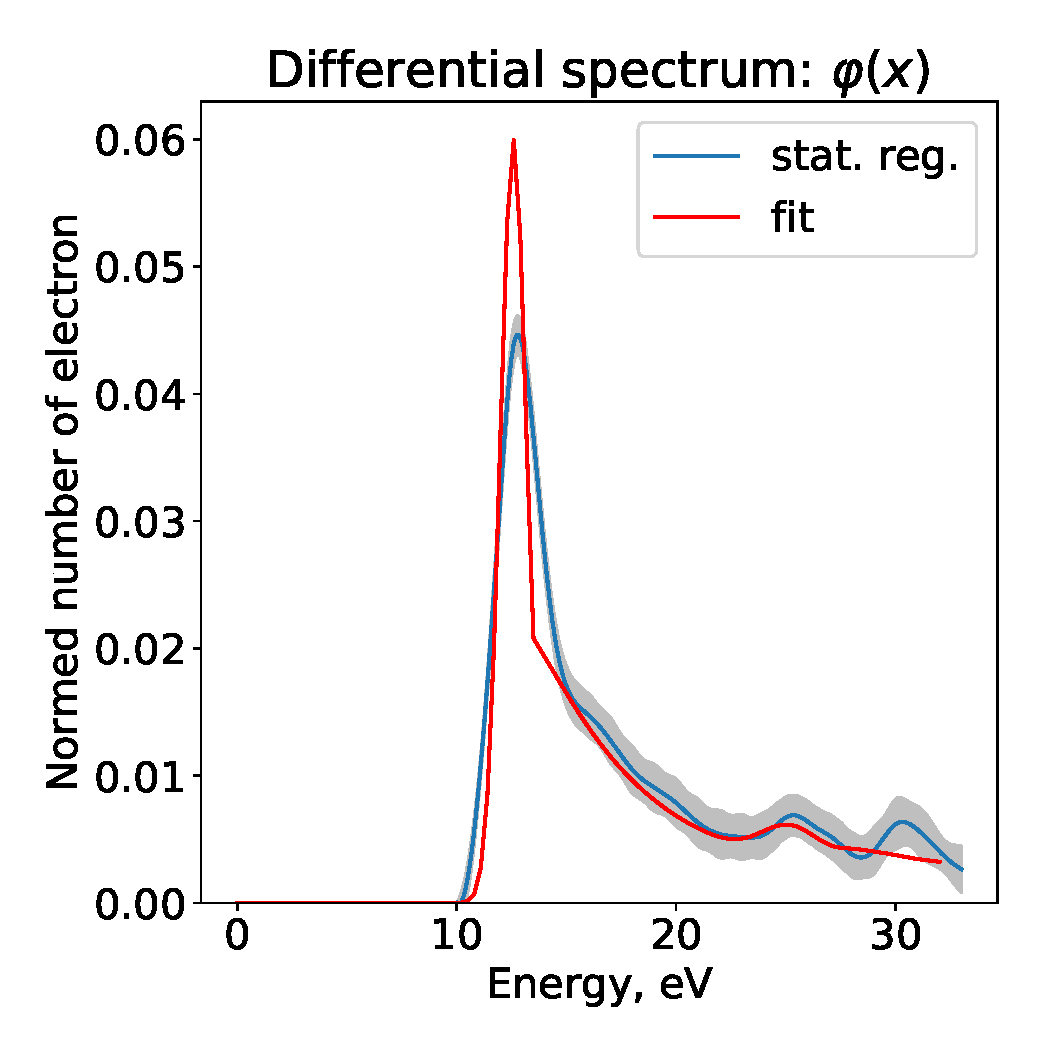
\includegraphics[width=0.95\textwidth]{image/fig02}
        \caption{}
        \label{pic-01-b}
    \end{subfigure}
    \caption{The spectrum of electron scattering (Troitsk $\nu$-mass data)}
\end{figure}

The basic concepts of the described method (alongside some improvements) were implemented in a new prototype program written in the Python language. Then the program was used to reconstruct the differential cross-sections of electron scattering on hydrogen isotopes measured in Troitsk nu-mass experiment. In this experiment gaseous hydrogen (as well as deuterium and tritium)  was irradiated by electrons with energies of about 20 keV from electron gun. Troitsk nu-mass spectrometer on the other side of gas volume registers the integral electron spectrum (like at fig~~\ref{pic-01-a}) with relative resolution of about $10^{-5}$. In previous works (\cite{Aseev2000} and \cite{Abdurashitov:2016nrv}) the differential cross-section of scattering electrons on $H2$ molecules was reconstructed using fit procedure against 5 or 6 parameters shape. That analysis had three major flaws:
\begin{itemize}
\item The parametric shape for fit does not have sufficient physics basis and therefore result is subjective in respect to the parametrization.
\item The chosen parametrization has too many parameters and produces very tight correlations between these parameters, making the fit results instable.
\item There is not clean way to determine uncertainties for any given point of reconstructed function.
\end{itemize}

Turchin's regularization allows to avoid all these problems and produces clean model-independent result with uncertainties. The result of regularization and previously published fit are presented at Fig.~\ref{pic-01-b}. The regularization reconstruction is in good agreement with fitted curve. Also there are two very small peaks picture shows two additional peaks at 25 and 30 eV.The peak on 25 eV is known to be produced by double scattering events. Peak on 30 eV is previously unknown. It could be either statistical anomaly (errors are quite large in this point), or possibly point to existence of additional dissociative scattering.

\section{Conclusion}

Turchin's statistical regularization is a very powerful tool to solve ill-posed inversed problems. It provides a flexible way to introduce almost any kind of prior knowledge into reconstruction problem. Also it opens a new way to solve some problems which previously were solved only by direct approach.
In this work, we created an implementation of Turchin's regularization using modern language and successfully applied it to the Troitsk nu-mass data for electron scattering on hydrogen isotopes. The work was preceded by a lot of testing of the algorithm with different artificial functions and discretization options. The results of those tests are beyond the scope of this article.

This work is supported by the Ministry of Education and Science of the Russian Federation under the contract No. 3.3008.2017/PP.

    
\bibliography{references}{}        
 
\end{document}
